\documentclass[12pt]{article}
\usepackage[utf8]{inputenc}
\usepackage[english]{babel}
\usepackage[letterpaper, portrait, margin=1in]{geometry}
\usepackage{amsmath}
\numberwithin{equation}{section}
\usepackage{amssymb}
\usepackage{graphicx}
\usepackage{parskip}
\usepackage{xcolor}
\usepackage{physics}
\usepackage{empheq}
\usepackage{cancel}
\usepackage{hyperref}
\hypersetup{colorlinks = true, urlcolor = blue, linkcolor = red, citecolor = red}
\usepackage{enumerate}
\usepackage{tikz}
\usepackage{float}
\usepackage{tcolorbox}
\usepackage{booktabs}
\usepackage[bottom]{footmisc}

% Default fixed font does not support bold face
\DeclareFixedFont{\ttb}{T1}{txtt}{bx}{n}{12} % for bold
\DeclareFixedFont{\ttm}{T1}{txtt}{m}{n}{12}  % for normal

% Custom colors
\usepackage{color}
\definecolor{deepblue}{rgb}{0,0,0.5}
\definecolor{deepred}{rgb}{0.6,0,0}
\definecolor{deepgreen}{rgb}{0,0.5,0}

\usepackage{listings}

% Python style for highlighting
\newcommand\pythonstyle{\lstset{
language=Python,
basicstyle=\ttm,
morekeywords={self},              % Add keywords here
commentstyle=\color{gray},
keywordstyle=\ttb\color{deepblue},
emph={MyClass,__init__},          % Custom highlighting
emphstyle=\ttb\color{deepred},    % Custom highlighting style
stringstyle=\color{deepgreen},                        % Any extra options here
showstringspaces=false
}}


% Python environment
\lstnewenvironment{python}[1][]
{
\pythonstyle
\lstset{#1}
}
{}

% Python for external files
\newcommand\pythonexternal[2][]{{
\pythonstyle
\lstinputlisting[#1]{#2}}}

% Python for inline
\newcommand\pythoninline[1]{{\pythonstyle\lstinline!#1!}}

\usepackage{xcolor}
\usepackage{fancyhdr}
\pagestyle{fancy}
\fancyhf{}
\fancyfoot[C]{\color{lightgray} Python Lecture VI Notes---Yi J Zhu}
\fancyfoot[L]{\color{lightgray} \today}
\fancyfoot[R]{Page \thepage}
\renewcommand{\headrulewidth}{0pt}
\renewcommand{\footrulewidth}{0pt}
\begin{document}

\section{Review}

\textbf{Last time:}
\begin{itemize}
    \item Numpy
    \item Questions?
    \item Today: Plotting with Matplotlib and Pandas 
\end{itemize}

\section{Matplotlib Intro}
\begin{itemize}

    \item Matplotlib (Matlab Plotting Library) is a package for creating plots and figures
    \item Importing matplotlib:
    \begin{python}
    import matplotlib.pyplot as plt
    \end{python}
    \begin{figure}[H]
	    \centering
	    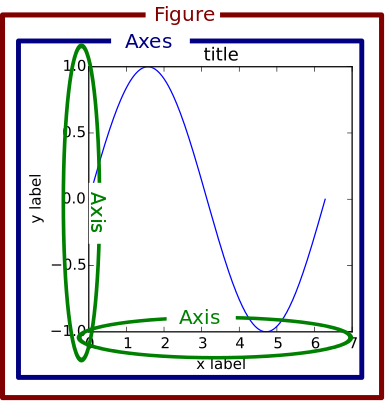
\includegraphics[width=7cm] {fig}
    \end{figure}
    \item \verb|Figure|: container for a matplotlib graphic. A figure contains multiple \verb|Axes| objects.
    \item \verb|Axes|: an individual plot. (Note: not be confused with AXIS).
    \item The \verb|Axes| contains the data to be plotted as well as the \verb|title, xlabel, legend| etc...
\end{itemize}

\section{A Basic Plot}
\begin{python}
fig, ax = plt.subplots(figsize=(8,6))

x = np.linspace(0, 10, 20)
y1 = 2*x+1
y2 = 3*x+1

ax.plot(x, y1, label='a line')
ax.plot(x, y2, label='a steeper line')
ax.set_title('A title!')
ax.set_xlabel('x')
ax.set_ylabel(r'$y = 2 \cdot x +1$')
ax.legend()

plt.show()
\end{python}

\begin{itemize}
    \item The \verb|pyplot.subplots| method creates and returns a \verb|Figure| and \verb|Axes|(s). \verb|pyplot| is a state-based interface: it retains a reference to the \verb|Figure| objected handed to you, so when you call \verb|pyplot|  later on, it knows which figures to make the changes.
    \item We can optionally specify the figure size in \verb|pyplot.subplots|.
    \item To populate the plot, we edit the \verb|Axes| object (\verb|ax|).
    \item We use the \verb|Axes.plot| method to plot our data. We can optionally specify a label
    \item \verb|Axes.set_title|, \verb|Axes.set_xlabel|, \verb|Axes.set_ylabel|, \verb|Axes.legend|
    \item In order to display the \verb|Figure|, we use the \verb|pyplot.show| function. This displays all open figures. After the show command, the displayed figures are closed (\verb|pyplot|'s internal state no longer tracks the figure).
\end{itemize}

\textbf{ax.plot format: }
\begin{itemize}
    \item \verb|ax.plot(x, y, [format])|
    \begin{figure}[H]
	    \centering
	    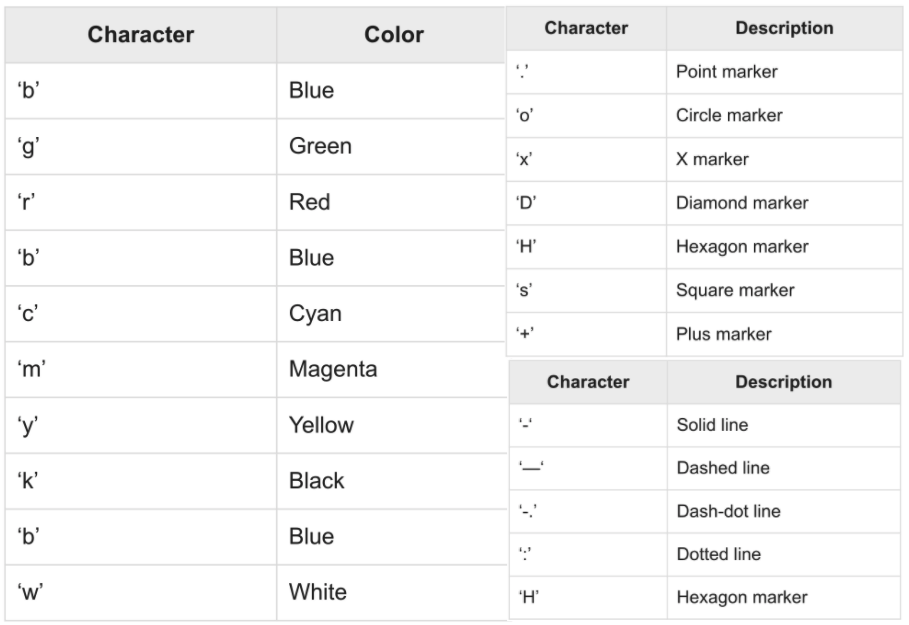
\includegraphics[width=12cm] {format}
    \end{figure}
    \item \verb|plot| has other properties, e.g. linewidth, markersize, etc...(read the docs)
\end{itemize}

\textbf{Additional Axes Methods (Demo)}:
\begin{itemize}
    \item \verb|Axes.grid()|
    \item \verb|Axes.set_xlim(min, max)|, \verb|Axes.set_ylim(min, max)|
    \item \verb|Axes.xscale(value)|, \verb|Axes.yscale(value)|, e.g. \verb|Axes.xscale(`log')|
    \item \verb|Axes.axhline(y)|, \verb|Axes.axvline(y)|
    \item \verb|Axes.errorbar(x, y, yerr=None, xerr=None, capsize=None)|
\end{itemize}

\textbf{Other types of plots} (read the docs):
\begin{itemize}
    \item Bar and Histogram
    \item Pie 
    \item Box and wisker
    \item etc...
\end{itemize}

\textbf{Histogram}
\begin{python}
x = np.random.normal(size=10000)
fig, ax = plt.subplots()
ax.hist(x, bins=30)
plt.show()
\end{python}
\begin{python}
x = np.random.uniform(size=10000)
fig, ax = plt.subplots()
ax.hist(x, bins=[0,0.1,0.2,0.3,0.6,0.7,0.8,0.9,1])
plt.show()
\end{python}
\begin{itemize}
	\item 
	\item
\end{itemize}

\section{Subplots}
\begin{itemize}
    \item Recall: we use the \verb|subplots| function to create a \verb|Figure|. By default, this creates one \verb|Axes|. However, we can specify a grid of \verb|Axes|: \verb|ax.subplots(rows, cols)|
    \item \verb|subplots| returns the figure and array of \verb|Axes|
    \item Example:
    \begin{python}
    fig, ax = plt.subplots(2, 3, figsize=(8,6))
    ax[0][1].plot(x,y1)
    ax[1][0].plot(x,y2)
    plt.show()
    \end{python}
    \item We can arrange the \verb|Axes| in more complicated manners. Read the docs...
\end{itemize}

\section{2D Plots}

\textbf{Plotting a 2d function: }$z(x,y) = x+y$

\begin{figure}[H]
	    \centering
	    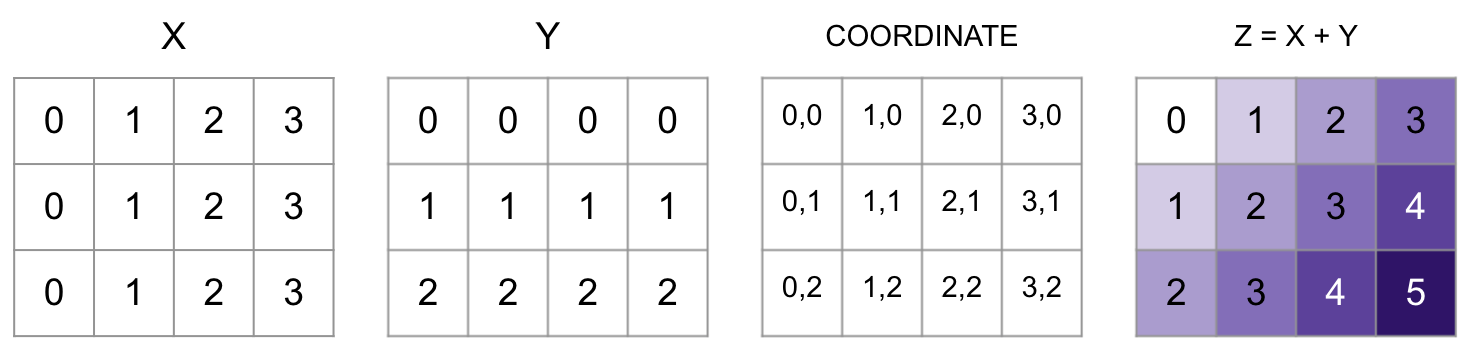
\includegraphics[width=15cm] {im}
\end{figure}

\begin{itemize}
    \item How do we generate $x$, $y$, and $z$? Numpy!
    \begin{python}
    x = np.arange(4)
    y = np.arange(3)
    X, Y = np.meshgrid(x,y)
    Z = X + Y
    
    >>> X
    array([[0, 1, 2, 3],
           [0, 1, 2, 3],
           [0, 1, 2, 3]])
    >>> Y
    array([[0, 0, 0, 0],
           [1, 1, 1, 1],
           [2, 2, 2, 2]])
    >>> Z
    array([[0, 1, 2, 3],
           [1, 2, 3, 4],
           [2, 3, 4, 5]])
    \end{python}
    \item Two ways to plot: \verb|imshow| and \verb|pcolormesh|
    \item \verb|imshow(Z)|: assumes values are equally spaced (for plotting images and 2d functions).
    \begin{verbatim}
                              +--------+--------+
                              | Z[0,0] | Z[0,1] |
                              +--------+--------+
                              | Z[1,0] | Z[1,1] |
                              +--------+--------+
    \end{verbatim}
    \item \verb|pcolormesh(X, Y, C)|: does not assumed equally spaced values. \verb|X| and \verb|Y| specify the quadrilateral corners. This is a mesh (cells do not have to be evenly spaced)!
    \begin{verbatim}
        (X[i+1, j], Y[i+1, j])          (X[i+1, j+1], Y[i+1, j+1])
                              +--------+
                              | C[i,j] |
                              +--------+
            (X[i, j], Y[i, j])          (X[i, j+1], Y[i, j+1]),
    \end{verbatim}
    \item We will use \verb|imshow|:
    \begin{python}
    fig, ax = plt.subplots(figsize=(8, 5))
    image = ax.imshow(Z)
    plt.show()
    \end{python}
    \item Color-map: key for how to map a value to a color. Matplotlib has many built-in cmaps and you can define your own.
    \begin{python}
    # default color map
    fig, ax = plt.subplots(figsize=(8, 5))
    image = ax.imshow(Z)
    plt.colorbar(image)
    plt.show()
    
    # example of a monotone cmap
    fig, ax = plt.subplots(figsize=(8, 5))
    image = ax.imshow(Z, cmap='Purples')
    plt.colorbar(image)
    plt.show()
    \end{python}
    \item We can also plot contours using \verb|ax.contour([X, Y], Z, [levels])|
\end{itemize}

\section{(Optional) Example: Plotting a Dipole Potential}
\textbf{Note}: this demo includes many optional arguments/features not covered in lecture. It's impossible cover nor remember everything. Searching the docs is an important skill!

\begin{python}
import matplotlib
x = np.linspace(-1.5, 1.5, 200)
y = np.linspace(-1, 1, 200)
X, Y = np.meshgrid(x,y)

# calculate dipole potential
R1 = np.sqrt((X-1)**2 + Y**2)
R2 = np.sqrt((X+1)**2 + Y**2)
Z = (1/R1 - 1/R2)
Z /= np.max(Z) # normalize

fig, ax = plt.subplots(figsize=(10, 7))
image = ax.imshow(Z, origin='lower', cmap='bwr',
                  extent=[np.min(x), np.max(x), np.min(y), np.max(y)],
                  norm=matplotlib.colors.SymLogNorm(0.01))
eqipots = [-0.1, -0.03, -0.01, -0.003, -0.001, 0, 
           0.001, 0.003, 0.01, 0.03, 0.1]
ax.contour(X, Y, Z, eqipots, colors='k')

ax.set_title('Dipole Potential', fontsize=16)
ax.set_xlabel(r'$x$', fontsize=16)
ax.set_ylabel(r'$y$', fontsize=16)

plt.colorbar(image, fraction=.03)
plt.savefig('dipole.png', dpi=300, bbox_inches='tight')
plt.show()
\end{python}

\begin{figure}[H]
    \centering
    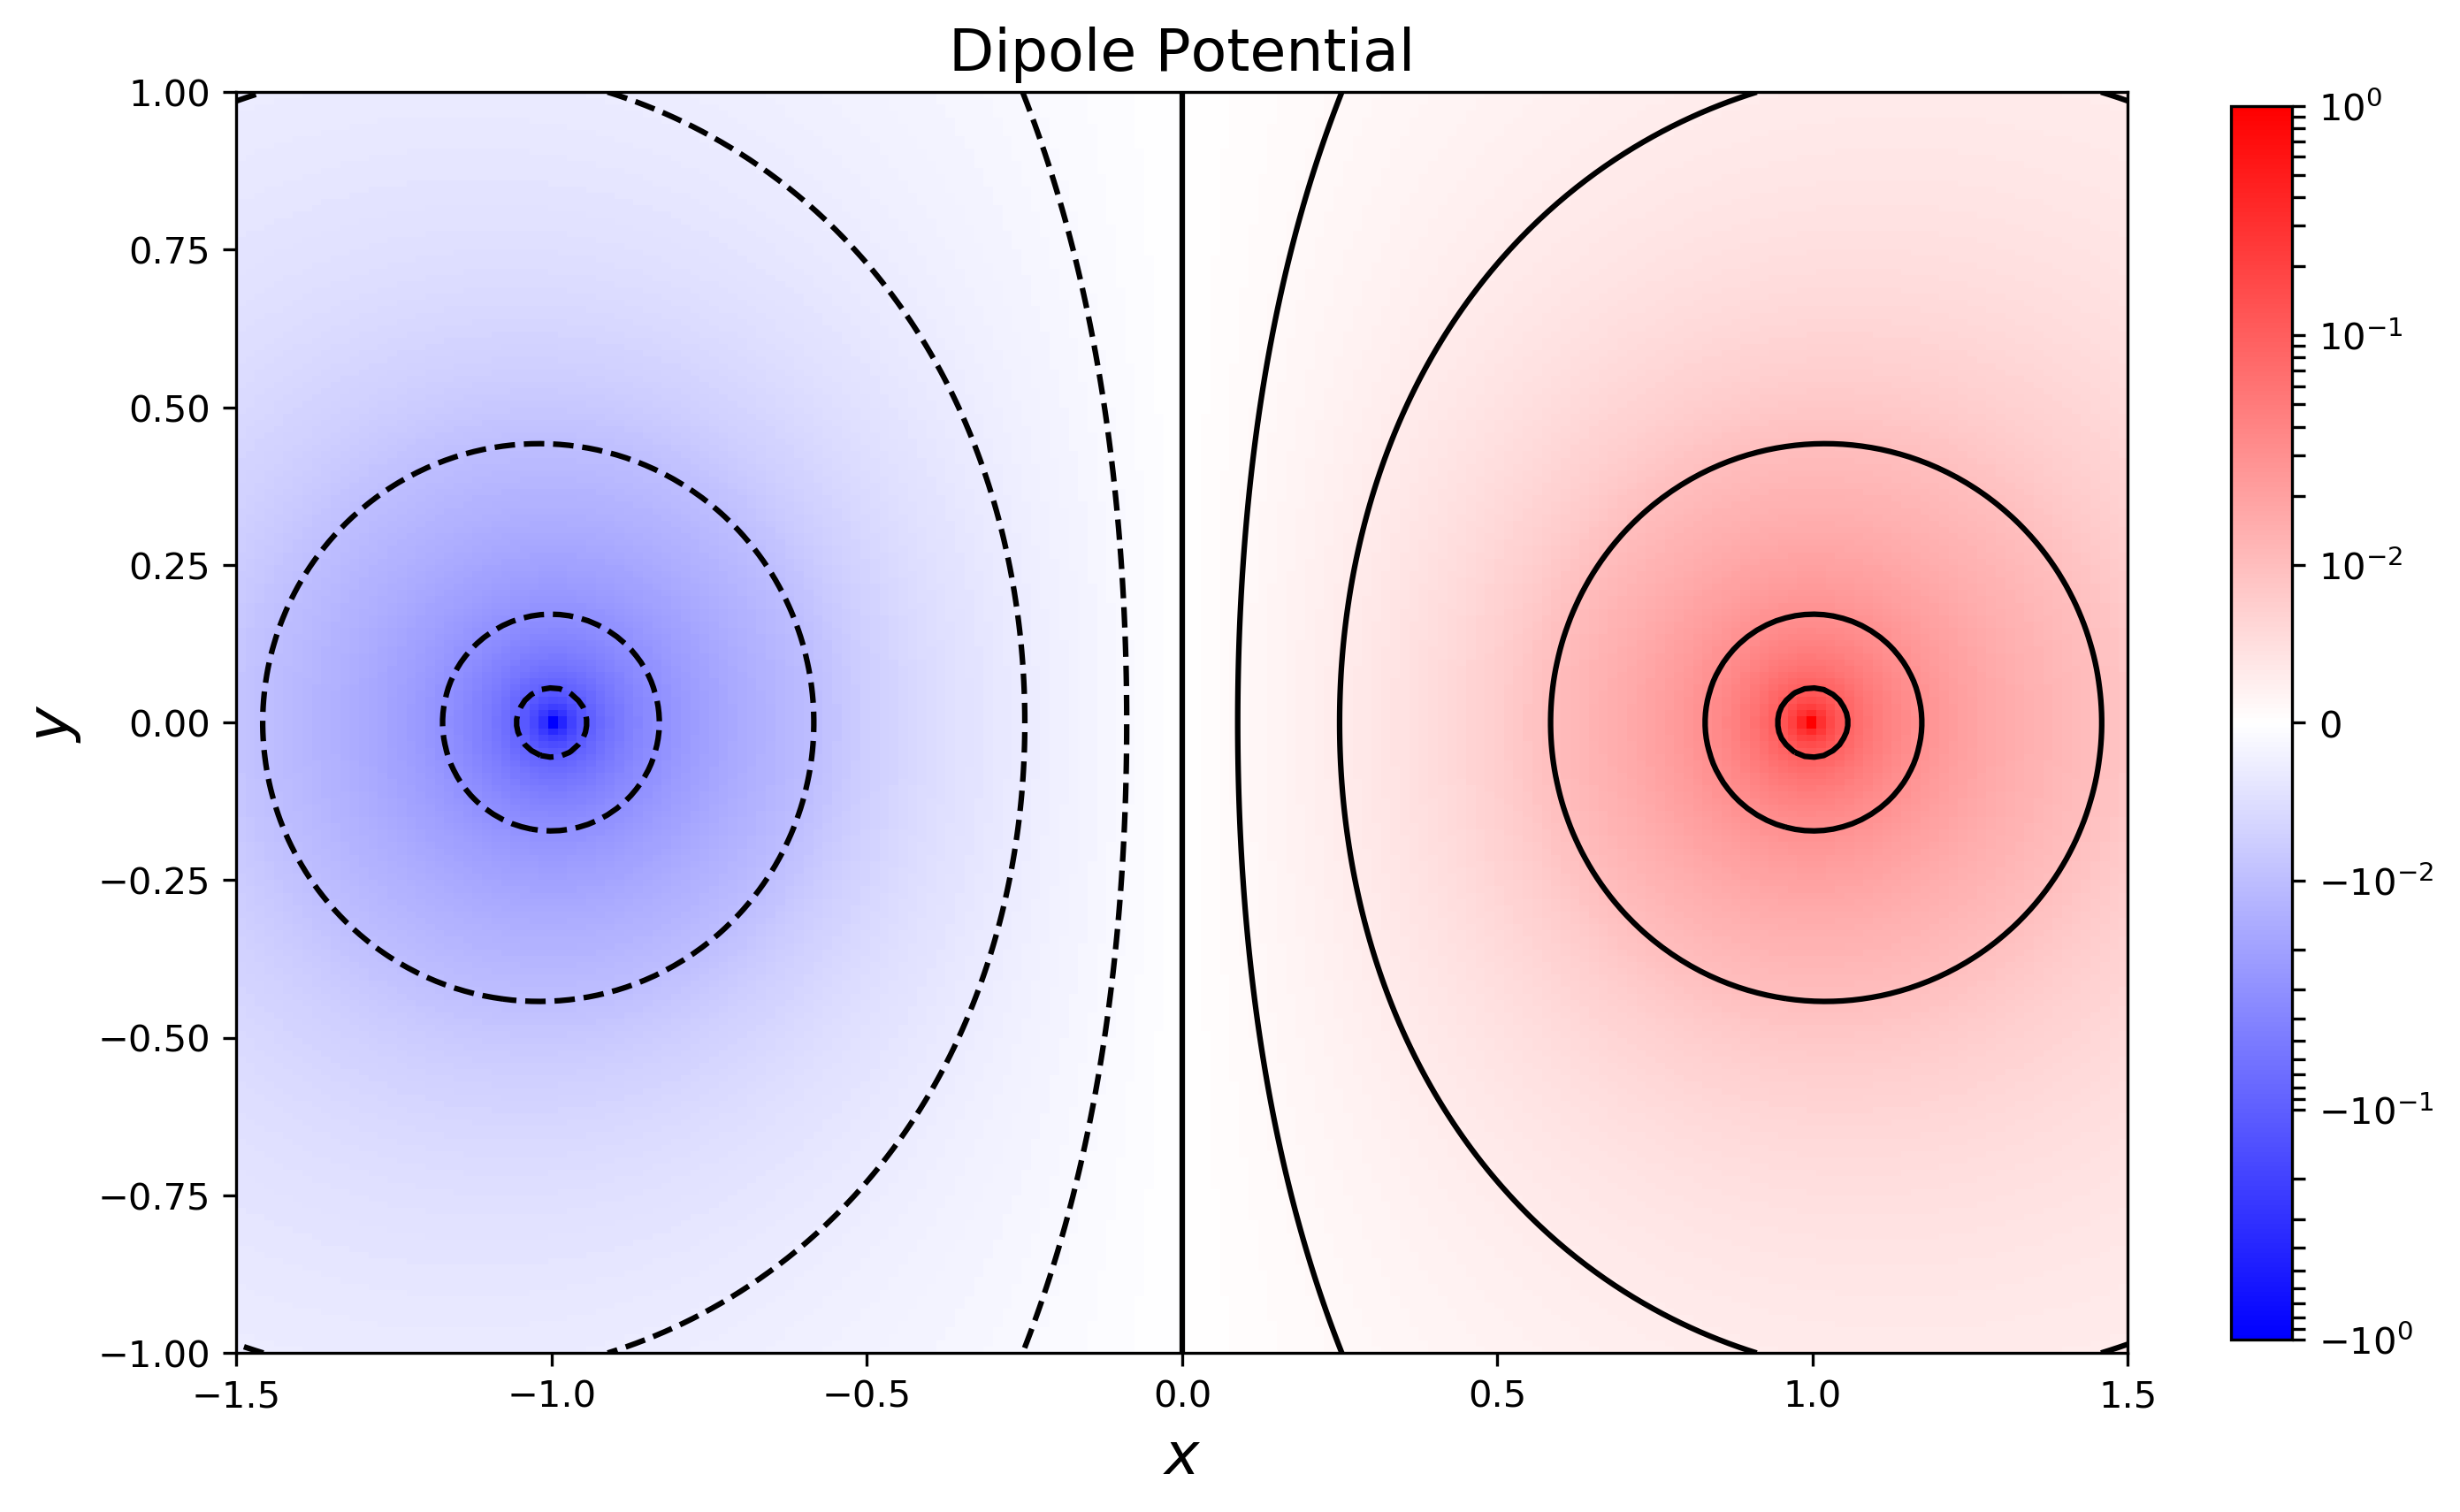
\includegraphics[width=16cm] {dipole}
\end{figure}

\section{Save Figure}
\begin{itemize}
    \item \verb|plt.savefig(name)|
    \item Recommend args: \verb|dpi=300, bbox_inches='tight'|
    \item If you want to show and save figure, you must save BEFORE showing
    \item Example:  
    \begin{python}
    plt.savefig('fig.png',dpi=300,bbox_inches='tight')
    \end{python}
\end{itemize}

\section{Pandas}
\begin{itemize}
    \item Pandas is a package for reading and cleaning data. This is a topic that could fill many lectures itself. I will only show a limited functionality.
    \item Reading in csv/txt file from computer/online (\verb|bb.txt| is included as a backup). Some common optional arguments for \verb|pd.read_csv|: \verb|header=None|, \verb|encoding = `utf8'|.
    \begin{python}
    import pandas as pd
    # data frame
    df = pd.read_csv('https://www.ocf.berkeley.edu/~yizhu/bb.txt',
                        delimiter=',', skiprows=0)
    
    lam = df['Lambda (nm)']
    I = df['Specific Intensity (W/m^3*Sr)']

    >>> df
             Lambda (nm)  Specific Intensity (W/m^3*Sr)
    0     300.000000                   7.940206e+12
    1     303.517588                   8.338975e+12
    2     307.035176                   8.756094e+12
    3     310.552764                   8.857883e+12
    4     314.070352                   9.422244e+12
    ..           ...                            ...
    195   985.929648                   9.643322e+12
    196   989.447236                   9.643796e+12
    197   992.964824                   9.547717e+12
    198   996.482412                   9.461644e+12
    199  1000.000000                   9.485265e+12
    
    [200 rows x 2 columns]
    
    >>>lam
    0       300.000000
    1       303.517588
    2       307.035176
    3       310.552764
    4       314.070352
              ...     
    195     985.929648
    196     989.447236
    197     992.964824
    198     996.482412
    199    1000.000000
    Name: Lambda (nm), Length: 200, dtype: float64
    \end{python}
	\item Data structures in \verb|pandas|: \verb|Series| and \verb|DataFrame|.
	\item \verb|Series|: a 1-dimensional ndarray of data. Each element in the series has a label (index). Example: \verb|lam| is a \verb|Series| indexed by 0, 1, 2, $\dots$. Indices do not have to be unique.
	\item \verb|DataFrame|: 2-dimension array storing tabular data. Tabular data is data arranged in a table form. Each row has the same columns as the other rows, in the same order. Each row is indexed by a label.
	\item Indexing data frames is a surprisingly complex topic. We will refer you to some resources from Data 100.
\end{itemize}

\section{Conclusion}
This is the end of the Python lecture series. This series is by no means comprehensive, but intended to prepare you to further learn/explore Python on your own. Remember:
\begin{itemize}
    \item Read the documentation
    \item Read the error tracebacks
    \item Google, StackOverflow, etc... is your friend
    \item Don't hesistate to reach out to the ULAB staff for help!
\end{itemize}

\end{document}
